% Author: Lukáš Ježek <xjezek19@stud.fit.vutbr.cz>


\documentclass[a4paper, 11pt]{article}


\usepackage[czech]{babel}

\usepackage[left=2cm, top=3cm, text={17cm, 24cm}]{geometry}
\usepackage{times}
\usepackage{graphicx}
\renewcommand{\rmdefault}{lmr}%zavede Latin Modern Roman jako rm / set Latin Modern Roman as rm
%---sf---------------
\renewcommand{\sfdefault}{qhv}%zavede TeX Gyre Heros jako sf
%---tt------------
\renewcommand{\ttdefault}{lmtt}% zavede Latin Modern tt jako tt
  \usepackage[unicode,colorlinks,hyperindex,plainpages=false,pdftex]{hyperref}
\hypersetup{
	colorlinks = true,
	hypertexnames = false,
	citecolor = blue
}


\fontfamily{qhv}\selectfont%

\begin{document}
	% Titulní stránka
	\begin{titlepage}
		\begin{center}
			
\includegraphics[width=0.77\linewidth]{FIT_logo.pdf} \\

			\vspace{\stretch{0.382}}

			\Huge{Projektová dokumentace} \\
			\LARGE{\textbf{
				Měření teploty
			}} \\
			\Large{IMP - Mikroprocesorové a vestavěné systémy}

			\vspace{\stretch{0.618}}
		\end{center}

		{\Large
			\today
			\hfill
			Lukáš Ježek (xjezek19)
		}
	\end{titlepage}



	% Obsah
	\pagenumbering{roman}
	\setcounter{page}{1}
	\tableofcontents
	\clearpage



	% Úvod
	\pagenumbering{arabic}
	\setcounter{page}{1}

	\section{Úvod}

Cílem projektu bylo vytvořit aplikaci pro zařízení ESP32, které dokáže měřit teplotu pomocí čidla LMT85LPG\footnote{\url{https://www.ti.com/lit/ds/symlink/lmt85.pdf}}, hodnoty ukládat s časovou značkou RTC, synchronizací s NTP serverem a přístupem k ovládání přes HTTP server. Použitý senzor poskytuje analogové údaje prostřednictvím hodnoty napětí v \texttt{mV} na jeho výstupu.

	% Návrh a implementace
\section{Zapojení a nastavení hardware}
 \subsection{Zapojení teplotního čidla}
 \label{temp_wiring}
 Teplotní čidlo obsahuje 3 konektory - napájení (3.3V), zem a výstupní analogový signál. Napájení bylo připojeno pomocí nepájivého pole na výstup ESP 3.3V a zem, pro data byl použit vstup ESP \texttt{GPIO36/ADC6} viz obrázek 1.
 \subsection{Zapojení LED diody}
 \label{led_wiring}
 Dioda obsahuje 2 konektory, katodu a anodu, na katodu jsem připojil předřazený odpor pro snížení vstupního napětí na \texttt{2V} namísto \texttt{3.3V}. Katodu jsem připojil k ESP \texttt{GPIO36} nakonfigurovaný jako výstup. Pro vypnutí diody je výstup v logické 1, pro rozsvícení naopak v logické 0.

\begin{figure}[h]
   \centering
    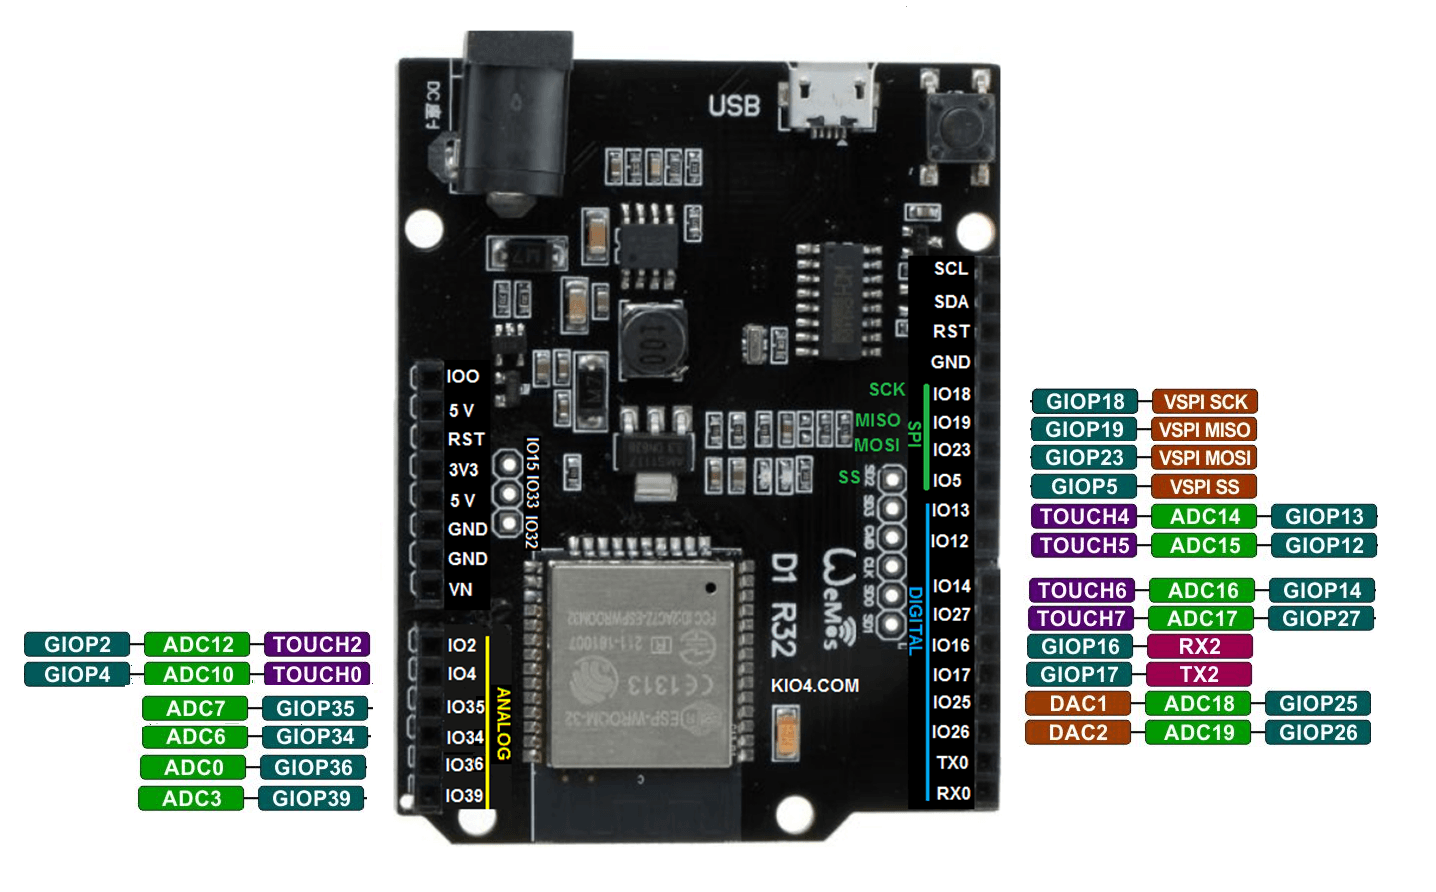
\includegraphics[width=\textwidth]{board.png}
 \caption{Schéma desky}
 \label{fig:Test}
\end{figure}

\begin{figure}[h]
   \centering
    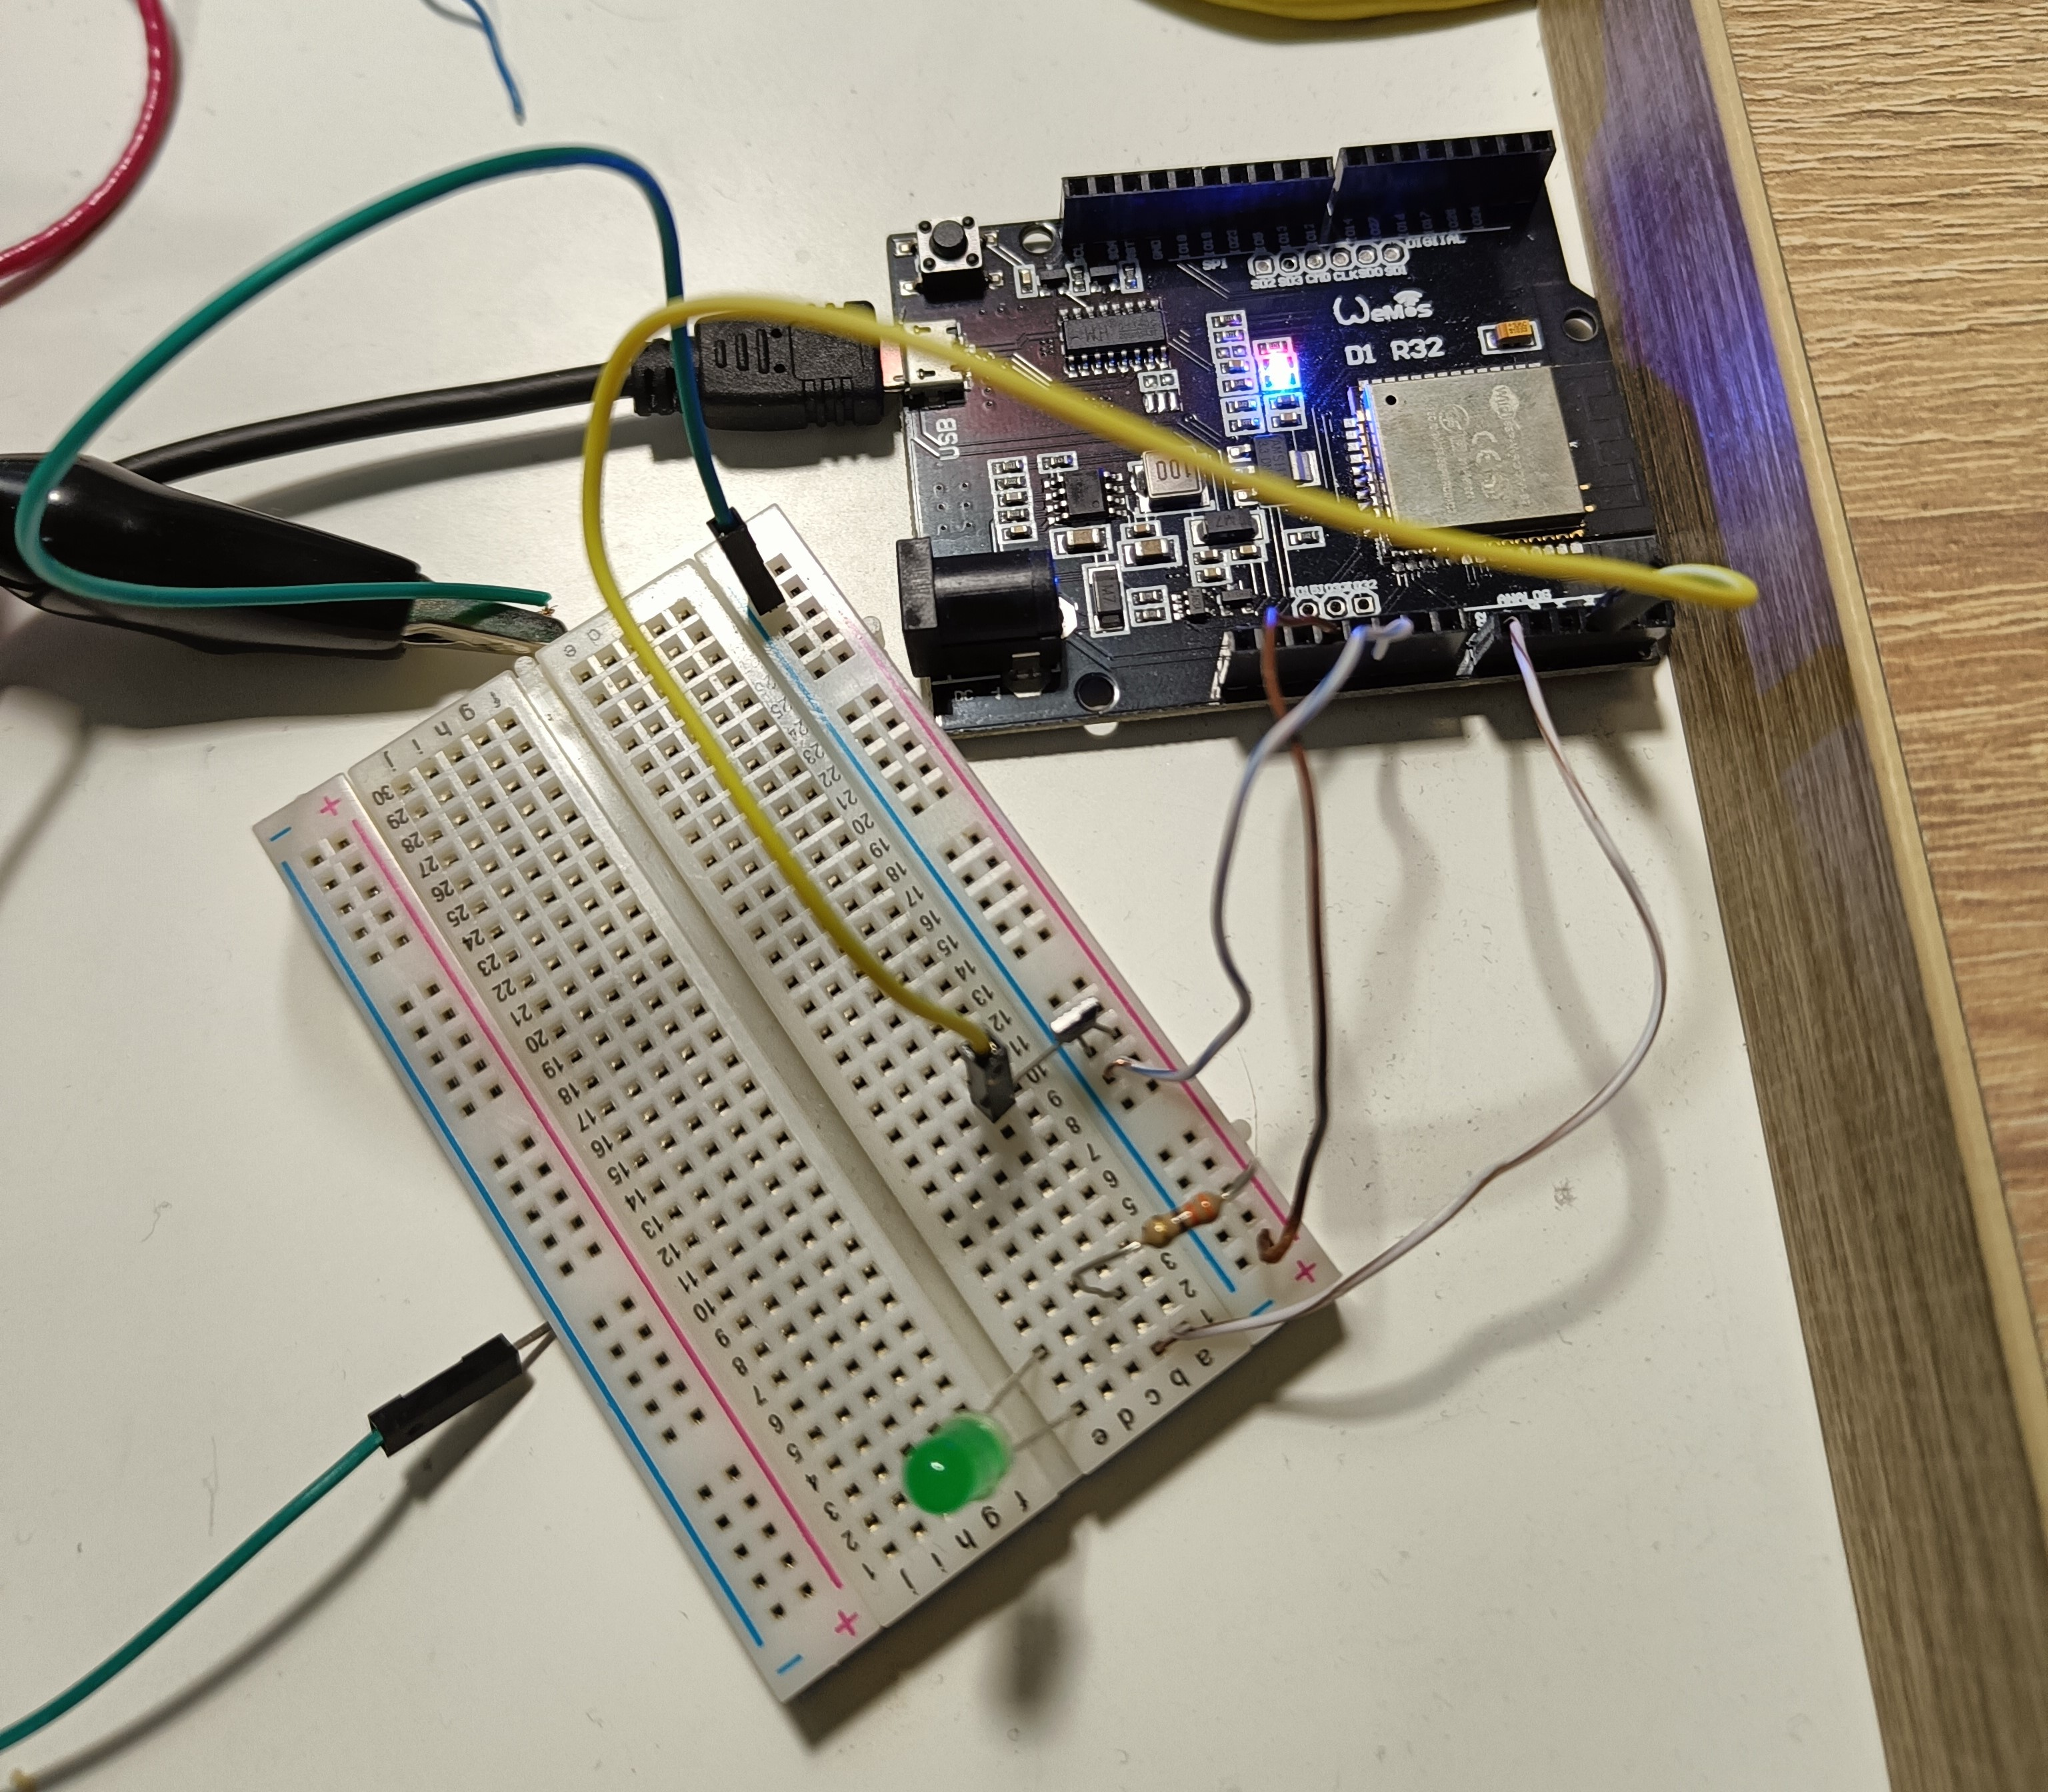
\includegraphics[width=\textwidth]{imp.jpg}
 \caption{Zapojení komponent}
 \label{fig:Test}
\end{figure}

	% Závěr
	\section{Řešení projektu}
 Aplikace je řešena pomocí IDF a Platformio. 
 \subsection{GPIO}
 Jako první po o spuštění samotného ESP, aplikace inicializuje GPIO, nastavením pinu pro LED diodu na mód \texttt{OUTPUT} a vypnutí \texttt{PULLUP a PULLDOWN}. Informaci o který GPIO pin se jedná můžeme změnit v \texttt{\#define LED\_PIN}.
 
 \subsection{Úložiště}
 Následně se začne inicializovat lokální úložiště pro ukládání historie měření. Jako úložiště se používá SPIFFS partition, nastavení pro platformio je uloženo v souboru partition.csv. Po inicializaci úložiště se provede kontrolní zápis do souboru, čímž se také vymaže veškerý jeho obsah obsah. V případě, že chceme zachovat měření i přes vypnutí, stačí změnit funkci \texttt{save\_string\_to\_file} na funkci \\ \texttt{append\_string\_to\_file}, která namísto otevření s parametrem \texttt{read} otevře soubor s parametrem \texttt{append} a pouze přidá další řádek. Obě tyto funkce jsou naimplementovány pomocí funkcí \texttt{fopen, fprintf, fclose}. V případě neúspěchu se vypíše příslušná chybová hláška na \texttt{ESP\_LOGE}.
 
 \subsection{Wifi}
 Další v pořadí inicializace je modul WiFi, který se pokusí připojit k nastavené síti ve zdrojovém kódu. Přístupové údaje k WiFi lze jednoduše změnit v souboru main.c pomocí deklarací \texttt{\#define WIFI\_SSID "název vaší wifi"} a \texttt{\#define WIFI\_PASS "heslo"}. Pro wifi je nutné inicializovat pamět NVS pomocí \texttt{nvs\_flash\_init()}. Inicializace wifi je implementována ve funkci \texttt{connect\_wifi()}, kde se zavede event loop a vytvoří se handlery pro wifi a pro získání IP adresy. Každý handler má svoji implementaci v samostatné funkci. Následně se zkontroluje výsledek připojení porovnáním bitů a případě se vypíše chybová hláška. Pokud se nepodaří připojit k zadané síti, aplikace opakuje ještě 15 pokusů o připojení, pokud se i tak nepodaří k síti připojit aplikace končí. V případě úspěchu a získání IP adresy zařízení vypíše přidělenou IP adresu a nastartuje webserver pro připojení na získané IP adrese. 

 \subsection{Webserver}
 Pokud se povede připojit k síti wifi, vytvoří se pomocí \texttt{xTaskCreate}\footnote{\url{https://www.freertos.org/a00125.html}} task pro provoz webserveru. Funkce přijímá jako handler funkci \texttt{http\_server\_task}, v této funkci jsou registrovány dostupné url pomocí \texttt{httpd\_register\_uri\_handler} a jednotlivých cest: \texttt{/} pro hlavní stránku - \texttt{root\_handler()}, \texttt{/historie.txt} pro textový soubor s logy teplot - \texttt{get\_file\_handler()}, \texttt{/submit} pro odeslání formuláře a přijetí dat -\texttt{submit\_handler()}, a \texttt{/\*} pro zobrazení 404 - výchozí \texttt{httpd\_resp\_send\_404}. Všechny metody jsou \texttt{GET}. Ve funkci \texttt{submit\_handler()} se z URL vyparsují znaky s informacemi a podle klíčů \texttt{value} a \texttt{hist} se vybere hodnota pro teplotu a histerzi. Do konzole se vypíše infromace o tom, že byla daná hodnota uložena, pokud je histerze menší než 0, hodnota se nastaví na 0. Funkce \texttt{get\_file\_hander()} otevře soubor \texttt{historie.txt} pro čtení a postupně pomocí \texttt{httpd\_resp\_send\_chunk()} zašle část dat ze souboru z bufferu o velikosti 1024, poté soubor uzavírá. Hlavní stránku zobrazuje \texttt{root\_handler}, ten nahradí proměnné v připravené HTML šabloně reálnými daty a zašle klientovi. Nazrazují se informace o aktuální teplotě, hodnoty prahové teploty a histerze.


\subsection{Měření teploty}
Další v pořadí se nastaví nakonfiguruje ADC převodník\footnote{\url{https://docs.espressif.com/projects/esp-idf/en/v4.4/esp32/api-reference/peripherals/adc.html#adc-api-reference-adc-driver}} pro získávání hodnot z teplotního čidla. Zde jsem narazil při kompilování na varování, že se jedná o zastaralou knihovnu a je vhodné ji nahradit knihovnou novější, ta mi však bohužel nefungovala a z toho důvodu jsem se rozhodl zůstat u této starší verze. Pro inicializaci jsem využil funkce \texttt{esp\_adc\_cal\_characterize()}, která zapíše kalibrační data do struktury \texttt{adc1\_chars} pro přesnější data. Pro převod hodnot z čidla jsem využil funkce \texttt{esp\_adc\_cal\_raw\_to\_voltage()} která tato data využívá pro přesnější získávání hodnot v \texttt{mV}. Výsledná teplota je potom vypočtena pomocí vztahu z dokumentace čidla \cite{cidloMan}[Strana 10].

\subsection{Synchronizace s NTP serverem}
Pro zápis do historie je třeba časová značka z doby pořízení zápisu, pro tento účel inicializuji čas ESP na výchozí hodnotu, kterou se následně pokusím aktualizovat pomocí volání na server \texttt{tik.cesnet.cz}, k tomu souží nastavení serveru v \texttt{esp\_sntp\_config\_t} a zavolání funkce \texttt{esp\_netif\_sntp\_init()} s touto strukturou a následně se pokusím kontaktovat server \texttt{esp\_netif\_sntp\_sync\_wait()} s časováním na max 15 vteřin, po té době se vypíše hláška o neúspěchu a pokračuje se v běhu programu. V případě úspěchu se opět vypíše hláška o úspěšné aktualizaci času.

 \subsection{LED Dioda}
 LED dioda je zapojená viz \ref{led_wiring}. Její ovládání spočívá v porovnání nastavené prahové teploty a histerze s reálnou hodnotou, pokud je  aktuální teplota nižší nebo rovna teplotě (nastavená - histerze), pak se dioda sepne, pokud je teplota vyšší než (nastavená + histerze) naopak se vypne. V případě, že je teplota mezi těmito hodnotami, s diodou se nic neděje a zůstává ve stejném stavu.

 \subsection{Hlavní smyčka}
 Po nastavení ADC převodníku se vstupuje do hlavní smyčky programu \texttt{while(1)}, kde se každý cyklus kontroluje naměřená hodnota z čidla, vypočítává se teplota, získává aktuální čas a vše se vypisuje na výstup, zároveň také zapisuje do souboru \texttt{historie.txt}. Poté smyčka vyčkává pomocí \texttt{vTaskDelay} 1 vteřinu a pokračuje v dalším cyklu.

 
    \section{Testování}
    Pro ověření hodnot jsem využíval multimetr a testování probíhalo pomocí vypisování debug výstupů do konzole. 
    
    \section{Závěr}
 
	Podařilo se mi implementovat všechny části aplikace, které byly uvedené v~zadání projektu. Při testování projektu jsem narazil pouze na nižší výstupní hodnotu z čidla, která byla následně zkalibrována na správný výsledek pomocí ESP. Celkově jsem nenarazil na žádné chybné chování programu, v pořádku proběhlo nastavení, nahrání, spuštění všech částí projektu i ovládání pomocí webserveru a ukládání historie dat. Čas zařízení je synchronizován ze serveru \texttt{tik.cesnet.cz}. Jako literaturu jsem použil zadanou studijní \cite{cidloMan} a dokumentaci pro ESP IDF \cite{espMan}. 

\section{Videa}
Pro předvedení fungování mého projektu jsem natočil 2 videa, krátké dle zadání, a dlouhé, ve kterém vysvětluji podrobněji fungování projektu. Budu rád za zhlédnutí. \url{https://nextcloud.fit.vutbr.cz/s/oTT3ZyjFBEWSytn}
	% Citace
	\clearpage
	\bibliographystyle{czechiso}
	\bibliography{manual}
\end{document}